\documentclass[UTF8]{ctexart}
\usepackage{mathtools,wallpaper}

\usepackage{t1enc}
\usepackage{pagecolor}
\usepackage{geometry}
\usepackage{diagbox}
\usepackage{graphicx}
\usepackage{wrapfig}

\geometry{left=2cm,right=2cm}

\begin{document}

\CTEXsetup[format={\Large\bfseries}]{section}
\title{实验报告}  
\author{徐亦昶 PB20000156}
\maketitle
\section{实验题目}重力加速度的测量
\section{实验目的}利用自由落体法和单摆法进行重力加速度的测量,并通过一系列措施改善测量的精度。
\section{自由落体法}
\subsection*{实验原理}
设加速度为g小球以速度$v_0$通过光电门1,经过时间$t_i$后到达
与光电门1相距$h_i$的光电门2,其中$i=1,2,\cdots n$,则有
\[h_1=v_0t_1+\frac{1}{2}gt_1^2\]
\[h_2=v_0t_2+\frac{1}{2}gt_2^2\]
\[\cdots\]
\[h_n=v_0t_n+\frac{1}{2}gt_n^2\]
即
\[\frac{h_1}{t_1}=v_0+\frac{1}{2}gt_1\]
\[\frac{h_2}{t_2}=v_0+\frac{1}{2}gt_2\]
\[\cdots\]
\[\frac{h_n}{t_n}=v_0+\frac{1}{2}gt_n\]
由于对每个i,$h_i$和$t_i$都是测量出的常数,因此可以通过线性拟合的方法
求出未知的参数$g$。在实验中,h和t分别用卷尺和双光电门法测出。
\subsection*{实验内容}
对大球、小球、圆柱分别进行下述实验:
\begin{enumerate}
    \item 将装置底座放在水平台面上,调整立柱底座的调节螺栓,使立柱竖直。
    \item 将一小球吸在立柱上端的电磁铁上,放置光电门1和光电门2。记录小球从
    断电到通过光电门1的时间差$t_{i1}$、从断电到通过光电门2的时间差$t_{i2}$以及小球通过两个光电门的时间差$t_{i}$。
    随后用$t_{i2}-t_{i1}$得到小球通过两个光电门的时间差,与
    之前测得的数值求平均得到$t_i$,移动光电门2。
    \item 用计算机或最小二乘法对$\frac{h_i}{t_i}=v_0+\frac{1}{2}gt_i$进行拟合,并求出所得直线的损失函数值
    \[loss\left( \hat{v_0},\hat{g} \right)=\sum_{i=1}^n\left(\frac{h_i}{t_i}-\hat{v_0}-\frac{1}{2}\hat{g}t_i\right)^2。\]
    \item $\hat{g}$即为重力加速度的估计值。
\end{enumerate}
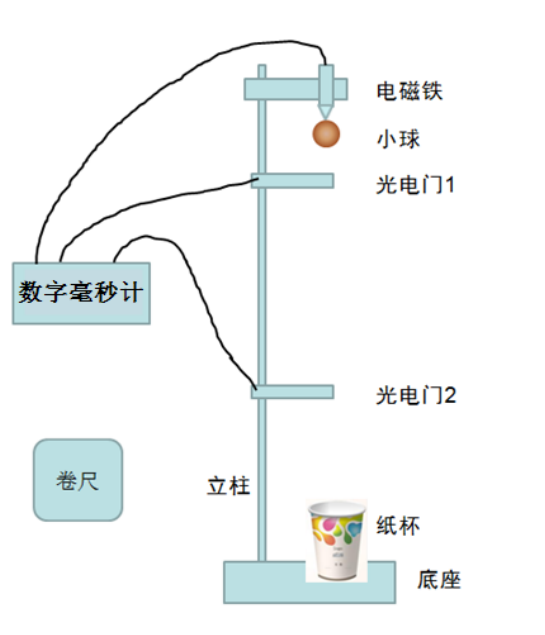
\includegraphics[scale=0.5]{fig1.PNG}
\newpage
\subsection*{数据记录}
\begin{table*}[htbp]
    \centering
    \fontsize{8}{10}\selectfont
    \caption{自由落体法测重力加速度(小球)}
    \scalebox{1.6}{
    \begin{tabular}{|c|c|c|c|c|c|c|}
    \hline
    \diagbox{测量参数}{实验次数i}& 1 & 2 & 3 & 4 & 5 & 6\\
    \hline
     $h_i/m$&0.500&0.450&0.400&0.350&0.300&0.250\\
     \hline
     $t_{i1}/s$&0.1685&0.1693&0.1683&0.1686&0.1686&0.1684\\
     \hline
     $t_{i2}/s$&0.3610&0.3484&0.3314&0.3159&0.2992&0.2825\\
     \hline
     $t_{i}/s$&0.1925&0.1791&0.1631&0.1473&0.1306&0.1141\\
     \hline
    \end{tabular}}
\end{table*}
\begin{table*}[htbp]
    \centering
    \fontsize{8}{10}\selectfont
    \caption{自由落体法测重力加速度(圆柱)}
    \scalebox{1.6}{
    \begin{tabular}{|c|c|c|c|c|c|c|c|c|}
    \hline
    \diagbox{测量参数}{实验次数i}& 1 & 2 & 3 & 4 & 5 & 6\\
    \hline
     $h_i/m$&0.500&0.450&0.400&0.350&0.300&0.250\\
     \hline
     $t_{i1}/s$&0.1732&0.1730&0.1729&0.1734&0.1732&0.1733\\
     \hline
     $t_{i2}/s$&0.3646&00.3498&0.3347&0.3204&0.3025&0.2855\\
     \hline
     $t_{i}/s$&0.1914&0.1768&0.1618&0.1470&0.1293&0.1122\\
     \hline
    \end{tabular}}
\end{table*}
\begin{table*}[htbp]
    \centering
    \fontsize{8}{10}\selectfont
    \caption{自由落体法测重力加速度(大球)}
    \scalebox{1.6}{
    \begin{tabular}{|c|c|c|c|c|c|c|}
    \hline
    \diagbox{测量参数}{实验次数i}& 1 & 2 & 3 & 4 & 5 & 6\\
    \hline
     $h_i/m$&0.500&0.450&0.400&0.350&0.300&0.250\\
     \hline
     $t_{i1}/s$&0.1661&0.1656&0.1659&0.1662&0.1661&0.1661\\
     \hline
     $t_{i2}/s$&0.3597&0.3441&0.3299&0.3135&0.2975&0.2797\\
     \hline
     $t_{i}/s$&0.1936&0.1785&0.1640&0.1473&0.1314&0.1136\\
     \hline
    \end{tabular}}
\end{table*}
\newpage
\subsection*{数据计算}
\subsubsection{小球下落数据计算}
求得重力加速度:$9.95m/s^2$
\newline 相关系数:r=0.9972972816880287
\begin{figure}[h]
    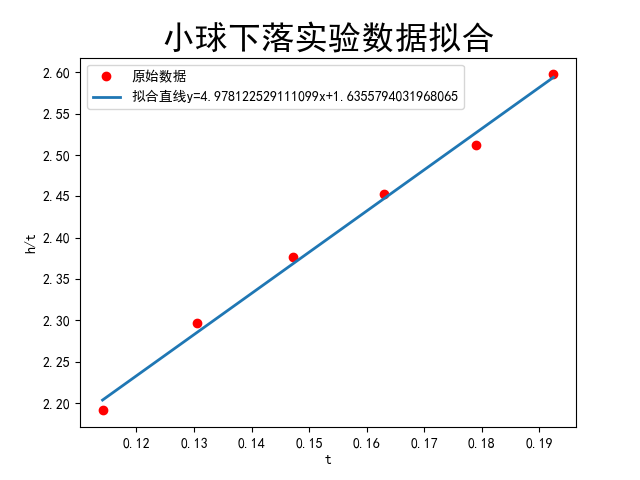
\includegraphics[scale=0.7]{data1_r=0.9972972816880287.png}
\end{figure}
\subsubsection{圆柱下落数据计算}
求得重力加速度:$9.70m/s^2$
\newline 相关系数:r=0.9982363750789983
\begin{figure}[h]
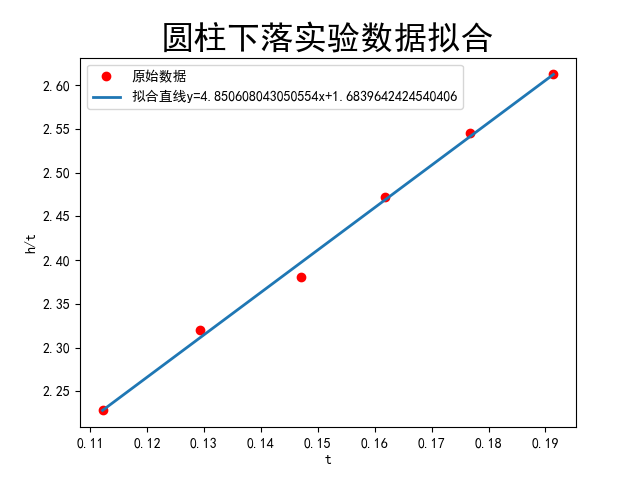
\includegraphics[scale=0.7]{data2_r=0.9982363750789983.png}
\end{figure}
\subsubsection{大球下落数据计算}
求得重力加速度:$9.62m/s^2$
\newline 相关系数:r=0.9987560595445574
\begin{figure}[h]
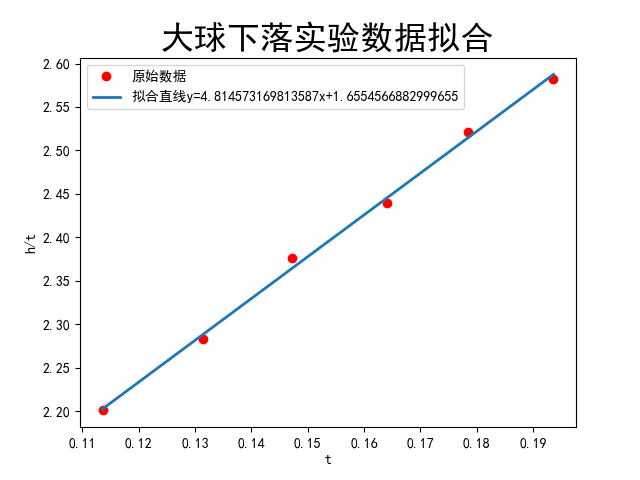
\includegraphics[scale=0.7]{data3_r=0.9987560595445574.png}
\end{figure}
\newpage
\subsection*{思考}
\begin{enumerate}
    \item 直接使用$h=\frac{1}{2}gt^2$很难难精确测量重力加速度。由于电磁铁有剩磁,因此小球
    下落的初始时间不准确。而本实验中通过两个时间相减的方法,避免了因计时延迟带来的误差。
    \item 为提高精度,各次实验中两光电门距离跨度应该尽可能大,这样可减小拟合时的误差。
    \item 通过本实验还可求出小球通过光电门1时的速度,用最小二乘法求出$v_0$即可。
    \item 显然可以使用$h=\frac{1}{2}gt^2$来进行不精确的测量,另外还有一种方法:
    调整光电门2的位置,使小球从下落至到达光电门2的时间为从下落至到达光电门1的时间的2倍,
    下落路程可用光电门1分成两段,第二段路程差-第一段路程差即为$gt^2$。如果支持再增加一个光电门,
    则使用三段路程中的下面两段进行如上计算,这样会更精确。
\end{enumerate}
\subsection{不确定度分析}
由实验数据得出,第一组值偏大,后两组g值偏小。第一组g值偏大的原因可能是
支架和地面不够垂直,后两组误差的主要来源是空气阻力,以及圆柱在空中的翻滚。
\section{单摆法}
\subsection*{实验原理}
单摆周期公式为
\[T=2\pi\sqrt{\frac{h}{g}\left[ 1+\frac{d^2}{20l^2}-\frac{m_0}{12m}\left( 1+\frac{d}{2l}+\frac{m_0}{m} \right)+\frac{\rho_0}{2\rho}+\frac{\theta^2}{16} \right]}\]
在实验精度要求在$10^{-3}$以内时,公式可近似为
\[T=2\pi\sqrt{\frac{l}{g}}\]
对$T^2g=4\pi^2l$两边微分,得到$2gdT^2+T^2dg=4\pi^2dl$,和$T^2g=4\pi^2l$相除,得到
$2\frac{dT^2}{T^2}+\frac{dg}{g}=4\pi^2\frac{dl}{l}$,当误差不大时,可近似为
\[2\frac{\Delta T^2}{T^2}+\frac{\Delta g}{g}=4\pi^2\frac{\Delta l}{l}\]
实验开始时,摆长为70cm,
若使用千分尺,则$4\pi^2\frac{\Delta l}{l}=4\pi^2\frac{10^{-5}}{0.7}=0.00112$,
又$2\frac{\Delta T^2}{T^2}\approx 2\times 0.014^2\div 1.4^2\approx 0.00028$,因此
用此方法测得的$\frac{\Delta g}{g}\approx 0.0014<0.01$。
故可以使用千分尺。
\subsection*{实验内容}
\begin{enumerate}
    \item 调节螺栓使立柱竖直,并调节标尺高度,使其上沿中点距
    悬挂点 70cm。
    \item 调整视线,使细线和平面镜中的镜像重合。
    \item 释放小球的同时计时,记录小球往返50个周期的时间T,由此得到一个平均周期。
    \item 重复上述步骤5次,取6次测得周期的平均值
    \item 求出重力加速度g。
    \item 实验结束,打乱支架平衡、标尺及平面镜位置。
\end{enumerate}
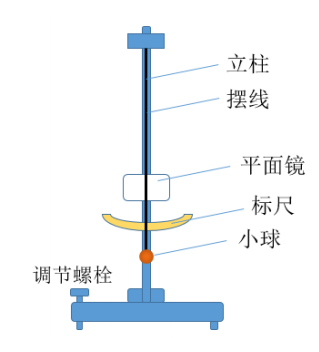
\includegraphics[scale=0.5]{fig2.PNG}
\subsection*{数据记录}
绳长:0.70m
\begin{table*}[hp]
    \centering
    \fontsize{8}{10}\selectfont
    \caption{单摆法测重力加速度}
    \scalebox{1.6}{
    \begin{tabular}{|c|c|c|c|c|c|c|}
    \hline
    \diagbox{测量参数}{实验次数i}& 1 & 2 & 3 & 4 & 5 & 6\\
    \hline
     50次周期$\left( s \right)/m$&84.27&84.30&84.27&84.29&84.28&84.31\\
     \hline
     单次周期$\left( s \right)/m$&1.68540&1.68600&1.68540&1.68580&1.68560&1.68620\\
     \hline
    \end{tabular}}
\end{table*}
\subsection*{数据计算}
求得的9.72478542802663$m/s^2$
\subsection*{不确定度分析}
\subsubsection*{A类不确定度}
$u_{AT}=\sqrt{\frac{\Sigma_{i=1}^6\left( T_i-\overline{T} \right)^2}{6\times 5}}=0.00013$
\[t_{0.68}=1.11\]
\subsubsection*{B类不确定度}
千分尺最大允差为0.001cm,估计误差为0.0005cm,因此$u_{Bl}=\sqrt{10^{-4}+25*10^{-8}}/3=0.00334$。
秒表最大允差为0.01s,估计误差为0.004s,B类不确定度的最大值$\Delta_{BT}=\sqrt{0.01^2+0.004^2}=0.01$
B类标准不确定度$u_{BT}=0.003$。对于秒表和千分尺,$k_{0.683}=1.000$,因此B类展伸不确定度均和B类标准不确定度
相等。因此$U_{0.68,l}=0.00334$,$U_{0.68,T}=0.00300$,根据不确定度传递公式
\[U_{0.68,g}=\sqrt{\left(  \frac{4\pi^2}{T^2}\right)^2U_{0.48,l}^2-\left(  \frac{8\pi^2l}{T^3}\right)^2U_{0.68,T}^2}\],
可得$U_{0.68,g}=0.03$。因此$g=9.725\pm 0.03m/s^2$。
\subsection*{思考}
本实验误差主要有两个:其一是由于操作不精确,任意使球做圆锥摆运动,从而导致测得的周期偏长,g值偏小;
其二是秒表计时不够准确。对于第一个问题可以使用尺子等拨动小球,使其保持在一平面内运动。
或者更精确地,可以使用电磁铁控制小球的下摆。对于第二个问题,可以增加周期数并求平均值,或者使用
光电门,这样也避免了因视线左移或右移造成的误差。
\end{document}